
% Default to the notebook output style

    


% Inherit from the specified cell style.




    
\documentclass[11pt,french]{article}
	\usepackage{babel}
    \usepackage[T1]{fontenc}
    \usepackage{array}
    % Nicer default font (+ math font) than Computer Modern for most use cases
    \usepackage{mathpazo}

    % Basic figure setup, for now with no caption control since it's done
    % automatically by Pandoc (which extracts ![](path) syntax from Markdown).
    \usepackage{graphicx}
    % We will generate all images so they have a width \maxwidth. This means
    % that they will get their normal width if they fit onto the page, but
    % are scaled down if they would overflow the margins.
    \makeatletter
    \def\maxwidth{\ifdim\Gin@nat@width>\linewidth\linewidth
    \else\Gin@nat@width\fi}
    \makeatother
    \let\Oldincludegraphics\includegraphics
    % Set max figure width to be 80% of text width, for now hardcoded.
    \renewcommand{\includegraphics}[1]{\Oldincludegraphics[width=.8\maxwidth]{#1}}
    % Ensure that by default, figures have no caption (until we provide a
    % proper Figure object with a Caption API and a way to capture that
    % in the conversion process - todo).
    \usepackage{caption}
    \DeclareCaptionLabelFormat{nolabel}{}
    \captionsetup{labelformat=nolabel}

    \usepackage{adjustbox} % Used to constrain images to a maximum size 
    \usepackage{xcolor} % Allow colors to be defined
    \usepackage{enumerate} % Needed for markdown enumerations to work
    \usepackage{geometry} % Used to adjust the document margins
    \usepackage{amsmath} % Equations
    \usepackage{amssymb} % Equations
    \usepackage{textcomp} % defines textquotesingle
    % Hack from http://tex.stackexchange.com/a/47451/13684:
    \AtBeginDocument{%
        \def\PYZsq{\textquotesingle}% Upright quotes in Pygmentized code
    }
    \usepackage{upquote} % Upright quotes for verbatim code
    \usepackage{eurosym} % defines \euro
    \usepackage[mathletters]{ucs} % Extended unicode (utf-8) support
    \usepackage[utf8x]{inputenc} % Allow utf-8 characters in the tex document
    \usepackage{fancyvrb} % verbatim replacement that allows latex
    \usepackage{grffile} % extends the file name processing of package graphics 
                         % to support a larger range 
    % The hyperref package gives us a pdf with properly built
    % internal navigation ('pdf bookmarks' for the table of contents,
    % internal cross-reference links, web links for URLs, etc.)
    \usepackage{hyperref}
    \usepackage{longtable} % longtable support required by pandoc >1.10
    \usepackage{booktabs}  % table support for pandoc > 1.12.2
    \usepackage[inline]{enumitem} % IRkernel/repr support (it uses the enumerate* environment)
    \usepackage[normalem]{ulem} % ulem is needed to support strikethroughs (\sout)
                                % normalem makes italics be italics, not underlines
    \usepackage{mathrsfs}
    

    
    
    % Colors for the hyperref package
    \definecolor{urlcolor}{rgb}{0,.145,.698}
    \definecolor{linkcolor}{rgb}{.71,0.21,0.01}
    \definecolor{citecolor}{rgb}{.12,.54,.11}

    % ANSI colors
    \definecolor{ansi-black}{HTML}{3E424D}
    \definecolor{ansi-black-intense}{HTML}{282C36}
    \definecolor{ansi-red}{HTML}{E75C58}
    \definecolor{ansi-red-intense}{HTML}{B22B31}
    \definecolor{ansi-green}{HTML}{00A250}
    \definecolor{ansi-green-intense}{HTML}{007427}
    \definecolor{ansi-yellow}{HTML}{DDB62B}
    \definecolor{ansi-yellow-intense}{HTML}{B27D12}
    \definecolor{ansi-blue}{HTML}{208FFB}
    \definecolor{ansi-blue-intense}{HTML}{0065CA}
    \definecolor{ansi-magenta}{HTML}{D160C4}
    \definecolor{ansi-magenta-intense}{HTML}{A03196}
    \definecolor{ansi-cyan}{HTML}{60C6C8}
    \definecolor{ansi-cyan-intense}{HTML}{258F8F}
    \definecolor{ansi-white}{HTML}{C5C1B4}
    \definecolor{ansi-white-intense}{HTML}{A1A6B2}
    \definecolor{ansi-default-inverse-fg}{HTML}{FFFFFF}
    \definecolor{ansi-default-inverse-bg}{HTML}{000000}

    % commands and environments needed by pandoc snippets
    % extracted from the output of `pandoc -s`
    \providecommand{\tightlist}{%
      \setlength{\itemsep}{0pt}\setlength{\parskip}{0pt}}
    \DefineVerbatimEnvironment{Highlighting}{Verbatim}{commandchars=\\\{\}}
    % Add ',fontsize=\small' for more characters per line
    \newenvironment{Shaded}{}{}
    \newcommand{\KeywordTok}[1]{\textcolor[rgb]{0.00,0.44,0.13}{\textbf{{#1}}}}
    \newcommand{\DataTypeTok}[1]{\textcolor[rgb]{0.56,0.13,0.00}{{#1}}}
    \newcommand{\DecValTok}[1]{\textcolor[rgb]{0.25,0.63,0.44}{{#1}}}
    \newcommand{\BaseNTok}[1]{\textcolor[rgb]{0.25,0.63,0.44}{{#1}}}
    \newcommand{\FloatTok}[1]{\textcolor[rgb]{0.25,0.63,0.44}{{#1}}}
    \newcommand{\CharTok}[1]{\textcolor[rgb]{0.25,0.44,0.63}{{#1}}}
    \newcommand{\StringTok}[1]{\textcolor[rgb]{0.25,0.44,0.63}{{#1}}}
    \newcommand{\CommentTok}[1]{\textcolor[rgb]{0.38,0.63,0.69}{\textit{{#1}}}}
    \newcommand{\OtherTok}[1]{\textcolor[rgb]{0.00,0.44,0.13}{{#1}}}
    \newcommand{\AlertTok}[1]{\textcolor[rgb]{1.00,0.00,0.00}{\textbf{{#1}}}}
    \newcommand{\FunctionTok}[1]{\textcolor[rgb]{0.02,0.16,0.49}{{#1}}}
    \newcommand{\RegionMarkerTok}[1]{{#1}}
    \newcommand{\ErrorTok}[1]{\textcolor[rgb]{1.00,0.00,0.00}{\textbf{{#1}}}}
    \newcommand{\NormalTok}[1]{{#1}}
    
    % Additional commands for more recent versions of Pandoc
    \newcommand{\ConstantTok}[1]{\textcolor[rgb]{0.53,0.00,0.00}{{#1}}}
    \newcommand{\SpecialCharTok}[1]{\textcolor[rgb]{0.25,0.44,0.63}{{#1}}}
    \newcommand{\VerbatimStringTok}[1]{\textcolor[rgb]{0.25,0.44,0.63}{{#1}}}
    \newcommand{\SpecialStringTok}[1]{\textcolor[rgb]{0.73,0.40,0.53}{{#1}}}
    \newcommand{\ImportTok}[1]{{#1}}
    \newcommand{\DocumentationTok}[1]{\textcolor[rgb]{0.73,0.13,0.13}{\textit{{#1}}}}
    \newcommand{\AnnotationTok}[1]{\textcolor[rgb]{0.38,0.63,0.69}{\textbf{\textit{{#1}}}}}
    \newcommand{\CommentVarTok}[1]{\textcolor[rgb]{0.38,0.63,0.69}{\textbf{\textit{{#1}}}}}
    \newcommand{\VariableTok}[1]{\textcolor[rgb]{0.10,0.09,0.49}{{#1}}}
    \newcommand{\ControlFlowTok}[1]{\textcolor[rgb]{0.00,0.44,0.13}{\textbf{{#1}}}}
    \newcommand{\OperatorTok}[1]{\textcolor[rgb]{0.40,0.40,0.40}{{#1}}}
    \newcommand{\BuiltInTok}[1]{{#1}}
    \newcommand{\ExtensionTok}[1]{{#1}}
    \newcommand{\PreprocessorTok}[1]{\textcolor[rgb]{0.74,0.48,0.00}{{#1}}}
    \newcommand{\AttributeTok}[1]{\textcolor[rgb]{0.49,0.56,0.16}{{#1}}}
    \newcommand{\InformationTok}[1]{\textcolor[rgb]{0.38,0.63,0.69}{\textbf{\textit{{#1}}}}}
    \newcommand{\WarningTok}[1]{\textcolor[rgb]{0.38,0.63,0.69}{\textbf{\textit{{#1}}}}}
    
    
    % Define a nice break command that doesn't care if a line doesn't already
    % exist.
    \def\br{\hspace*{\fill} \\* }
    % Math Jax compatibility definitions
    \def\gt{>}
    \def\lt{<}
    \let\Oldtex\TeX
    \let\Oldlatex\LaTeX
    \renewcommand{\TeX}{\textrm{\Oldtex}}
    \renewcommand{\LaTeX}{\textrm{\Oldlatex}}
    % Document parameters
    % Document title
    \title{Expressions booléennes}
    
    
    
    
    

    % Pygments definitions
    
\makeatletter
\def\PY@reset{\let\PY@it=\relax \let\PY@bf=\relax%
    \let\PY@ul=\relax \let\PY@tc=\relax%
    \let\PY@bc=\relax \let\PY@ff=\relax}
\def\PY@tok#1{\csname PY@tok@#1\endcsname}
\def\PY@toks#1+{\ifx\relax#1\empty\else%
    \PY@tok{#1}\expandafter\PY@toks\fi}
\def\PY@do#1{\PY@bc{\PY@tc{\PY@ul{%
    \PY@it{\PY@bf{\PY@ff{#1}}}}}}}
\def\PY#1#2{\PY@reset\PY@toks#1+\relax+\PY@do{#2}}

\expandafter\def\csname PY@tok@w\endcsname{\def\PY@tc##1{\textcolor[rgb]{0.73,0.73,0.73}{##1}}}
\expandafter\def\csname PY@tok@c\endcsname{\let\PY@it=\textit\def\PY@tc##1{\textcolor[rgb]{0.25,0.50,0.50}{##1}}}
\expandafter\def\csname PY@tok@cp\endcsname{\def\PY@tc##1{\textcolor[rgb]{0.74,0.48,0.00}{##1}}}
\expandafter\def\csname PY@tok@k\endcsname{\let\PY@bf=\textbf\def\PY@tc##1{\textcolor[rgb]{0.00,0.50,0.00}{##1}}}
\expandafter\def\csname PY@tok@kp\endcsname{\def\PY@tc##1{\textcolor[rgb]{0.00,0.50,0.00}{##1}}}
\expandafter\def\csname PY@tok@kt\endcsname{\def\PY@tc##1{\textcolor[rgb]{0.69,0.00,0.25}{##1}}}
\expandafter\def\csname PY@tok@o\endcsname{\def\PY@tc##1{\textcolor[rgb]{0.40,0.40,0.40}{##1}}}
\expandafter\def\csname PY@tok@ow\endcsname{\let\PY@bf=\textbf\def\PY@tc##1{\textcolor[rgb]{0.67,0.13,1.00}{##1}}}
\expandafter\def\csname PY@tok@nb\endcsname{\def\PY@tc##1{\textcolor[rgb]{0.00,0.50,0.00}{##1}}}
\expandafter\def\csname PY@tok@nf\endcsname{\def\PY@tc##1{\textcolor[rgb]{0.00,0.00,1.00}{##1}}}
\expandafter\def\csname PY@tok@nc\endcsname{\let\PY@bf=\textbf\def\PY@tc##1{\textcolor[rgb]{0.00,0.00,1.00}{##1}}}
\expandafter\def\csname PY@tok@nn\endcsname{\let\PY@bf=\textbf\def\PY@tc##1{\textcolor[rgb]{0.00,0.00,1.00}{##1}}}
\expandafter\def\csname PY@tok@ne\endcsname{\let\PY@bf=\textbf\def\PY@tc##1{\textcolor[rgb]{0.82,0.25,0.23}{##1}}}
\expandafter\def\csname PY@tok@nv\endcsname{\def\PY@tc##1{\textcolor[rgb]{0.10,0.09,0.49}{##1}}}
\expandafter\def\csname PY@tok@no\endcsname{\def\PY@tc##1{\textcolor[rgb]{0.53,0.00,0.00}{##1}}}
\expandafter\def\csname PY@tok@nl\endcsname{\def\PY@tc##1{\textcolor[rgb]{0.63,0.63,0.00}{##1}}}
\expandafter\def\csname PY@tok@ni\endcsname{\let\PY@bf=\textbf\def\PY@tc##1{\textcolor[rgb]{0.60,0.60,0.60}{##1}}}
\expandafter\def\csname PY@tok@na\endcsname{\def\PY@tc##1{\textcolor[rgb]{0.49,0.56,0.16}{##1}}}
\expandafter\def\csname PY@tok@nt\endcsname{\let\PY@bf=\textbf\def\PY@tc##1{\textcolor[rgb]{0.00,0.50,0.00}{##1}}}
\expandafter\def\csname PY@tok@nd\endcsname{\def\PY@tc##1{\textcolor[rgb]{0.67,0.13,1.00}{##1}}}
\expandafter\def\csname PY@tok@s\endcsname{\def\PY@tc##1{\textcolor[rgb]{0.73,0.13,0.13}{##1}}}
\expandafter\def\csname PY@tok@sd\endcsname{\let\PY@it=\textit\def\PY@tc##1{\textcolor[rgb]{0.73,0.13,0.13}{##1}}}
\expandafter\def\csname PY@tok@si\endcsname{\let\PY@bf=\textbf\def\PY@tc##1{\textcolor[rgb]{0.73,0.40,0.53}{##1}}}
\expandafter\def\csname PY@tok@se\endcsname{\let\PY@bf=\textbf\def\PY@tc##1{\textcolor[rgb]{0.73,0.40,0.13}{##1}}}
\expandafter\def\csname PY@tok@sr\endcsname{\def\PY@tc##1{\textcolor[rgb]{0.73,0.40,0.53}{##1}}}
\expandafter\def\csname PY@tok@ss\endcsname{\def\PY@tc##1{\textcolor[rgb]{0.10,0.09,0.49}{##1}}}
\expandafter\def\csname PY@tok@sx\endcsname{\def\PY@tc##1{\textcolor[rgb]{0.00,0.50,0.00}{##1}}}
\expandafter\def\csname PY@tok@m\endcsname{\def\PY@tc##1{\textcolor[rgb]{0.40,0.40,0.40}{##1}}}
\expandafter\def\csname PY@tok@gh\endcsname{\let\PY@bf=\textbf\def\PY@tc##1{\textcolor[rgb]{0.00,0.00,0.50}{##1}}}
\expandafter\def\csname PY@tok@gu\endcsname{\let\PY@bf=\textbf\def\PY@tc##1{\textcolor[rgb]{0.50,0.00,0.50}{##1}}}
\expandafter\def\csname PY@tok@gd\endcsname{\def\PY@tc##1{\textcolor[rgb]{0.63,0.00,0.00}{##1}}}
\expandafter\def\csname PY@tok@gi\endcsname{\def\PY@tc##1{\textcolor[rgb]{0.00,0.63,0.00}{##1}}}
\expandafter\def\csname PY@tok@gr\endcsname{\def\PY@tc##1{\textcolor[rgb]{1.00,0.00,0.00}{##1}}}
\expandafter\def\csname PY@tok@ge\endcsname{\let\PY@it=\textit}
\expandafter\def\csname PY@tok@gs\endcsname{\let\PY@bf=\textbf}
\expandafter\def\csname PY@tok@gp\endcsname{\let\PY@bf=\textbf\def\PY@tc##1{\textcolor[rgb]{0.00,0.00,0.50}{##1}}}
\expandafter\def\csname PY@tok@go\endcsname{\def\PY@tc##1{\textcolor[rgb]{0.53,0.53,0.53}{##1}}}
\expandafter\def\csname PY@tok@gt\endcsname{\def\PY@tc##1{\textcolor[rgb]{0.00,0.27,0.87}{##1}}}
\expandafter\def\csname PY@tok@err\endcsname{\def\PY@bc##1{\setlength{\fboxsep}{0pt}\fcolorbox[rgb]{1.00,0.00,0.00}{1,1,1}{\strut ##1}}}
\expandafter\def\csname PY@tok@kc\endcsname{\let\PY@bf=\textbf\def\PY@tc##1{\textcolor[rgb]{0.00,0.50,0.00}{##1}}}
\expandafter\def\csname PY@tok@kd\endcsname{\let\PY@bf=\textbf\def\PY@tc##1{\textcolor[rgb]{0.00,0.50,0.00}{##1}}}
\expandafter\def\csname PY@tok@kn\endcsname{\let\PY@bf=\textbf\def\PY@tc##1{\textcolor[rgb]{0.00,0.50,0.00}{##1}}}
\expandafter\def\csname PY@tok@kr\endcsname{\let\PY@bf=\textbf\def\PY@tc##1{\textcolor[rgb]{0.00,0.50,0.00}{##1}}}
\expandafter\def\csname PY@tok@bp\endcsname{\def\PY@tc##1{\textcolor[rgb]{0.00,0.50,0.00}{##1}}}
\expandafter\def\csname PY@tok@fm\endcsname{\def\PY@tc##1{\textcolor[rgb]{0.00,0.00,1.00}{##1}}}
\expandafter\def\csname PY@tok@vc\endcsname{\def\PY@tc##1{\textcolor[rgb]{0.10,0.09,0.49}{##1}}}
\expandafter\def\csname PY@tok@vg\endcsname{\def\PY@tc##1{\textcolor[rgb]{0.10,0.09,0.49}{##1}}}
\expandafter\def\csname PY@tok@vi\endcsname{\def\PY@tc##1{\textcolor[rgb]{0.10,0.09,0.49}{##1}}}
\expandafter\def\csname PY@tok@vm\endcsname{\def\PY@tc##1{\textcolor[rgb]{0.10,0.09,0.49}{##1}}}
\expandafter\def\csname PY@tok@sa\endcsname{\def\PY@tc##1{\textcolor[rgb]{0.73,0.13,0.13}{##1}}}
\expandafter\def\csname PY@tok@sb\endcsname{\def\PY@tc##1{\textcolor[rgb]{0.73,0.13,0.13}{##1}}}
\expandafter\def\csname PY@tok@sc\endcsname{\def\PY@tc##1{\textcolor[rgb]{0.73,0.13,0.13}{##1}}}
\expandafter\def\csname PY@tok@dl\endcsname{\def\PY@tc##1{\textcolor[rgb]{0.73,0.13,0.13}{##1}}}
\expandafter\def\csname PY@tok@s2\endcsname{\def\PY@tc##1{\textcolor[rgb]{0.73,0.13,0.13}{##1}}}
\expandafter\def\csname PY@tok@sh\endcsname{\def\PY@tc##1{\textcolor[rgb]{0.73,0.13,0.13}{##1}}}
\expandafter\def\csname PY@tok@s1\endcsname{\def\PY@tc##1{\textcolor[rgb]{0.73,0.13,0.13}{##1}}}
\expandafter\def\csname PY@tok@mb\endcsname{\def\PY@tc##1{\textcolor[rgb]{0.40,0.40,0.40}{##1}}}
\expandafter\def\csname PY@tok@mf\endcsname{\def\PY@tc##1{\textcolor[rgb]{0.40,0.40,0.40}{##1}}}
\expandafter\def\csname PY@tok@mh\endcsname{\def\PY@tc##1{\textcolor[rgb]{0.40,0.40,0.40}{##1}}}
\expandafter\def\csname PY@tok@mi\endcsname{\def\PY@tc##1{\textcolor[rgb]{0.40,0.40,0.40}{##1}}}
\expandafter\def\csname PY@tok@il\endcsname{\def\PY@tc##1{\textcolor[rgb]{0.40,0.40,0.40}{##1}}}
\expandafter\def\csname PY@tok@mo\endcsname{\def\PY@tc##1{\textcolor[rgb]{0.40,0.40,0.40}{##1}}}
\expandafter\def\csname PY@tok@ch\endcsname{\let\PY@it=\textit\def\PY@tc##1{\textcolor[rgb]{0.25,0.50,0.50}{##1}}}
\expandafter\def\csname PY@tok@cm\endcsname{\let\PY@it=\textit\def\PY@tc##1{\textcolor[rgb]{0.25,0.50,0.50}{##1}}}
\expandafter\def\csname PY@tok@cpf\endcsname{\let\PY@it=\textit\def\PY@tc##1{\textcolor[rgb]{0.25,0.50,0.50}{##1}}}
\expandafter\def\csname PY@tok@c1\endcsname{\let\PY@it=\textit\def\PY@tc##1{\textcolor[rgb]{0.25,0.50,0.50}{##1}}}
\expandafter\def\csname PY@tok@cs\endcsname{\let\PY@it=\textit\def\PY@tc##1{\textcolor[rgb]{0.25,0.50,0.50}{##1}}}

\def\PYZbs{\char`\\}
\def\PYZus{\char`\_}
\def\PYZob{\char`\{}
\def\PYZcb{\char`\}}
\def\PYZca{\char`\^}
\def\PYZam{\char`\&}
\def\PYZlt{\char`\<}
\def\PYZgt{\char`\>}
\def\PYZsh{\char`\#}
\def\PYZpc{\char`\%}
\def\PYZdl{\char`\$}
\def\PYZhy{\char`\-}
\def\PYZsq{\char`\'}
\def\PYZdq{\char`\"}
\def\PYZti{\char`\~}
% for compatibility with earlier versions
\def\PYZat{@}
\def\PYZlb{[}
\def\PYZrb{]}
\makeatother


    % Exact colors from NB
    \definecolor{incolor}{rgb}{0.0, 0.0, 0.5}
    \definecolor{outcolor}{rgb}{0.545, 0.0, 0.0}



    
    % Prevent overflowing lines due to hard-to-break entities
    \sloppy 
    % Setup hyperref package
    \hypersetup{
      breaklinks=true,  % so long urls are correctly broken across lines
      colorlinks=true,
      urlcolor=urlcolor,
      linkcolor=linkcolor,
      citecolor=citecolor,
      }
    % Slightly bigger margins than the latex defaults
    
    \geometry{verbose,tmargin=1in,bmargin=1in,lmargin=1in,rmargin=1in}
    
    
	\author{\textsc{Bruno Darid}}
    \begin{document}
  	\renewcommand{\contentsname}{\textsc{Plan}}    
 	\maketitle
 	\tableofcontents
    \newpage
    \hypertarget{repuxe8res-historiques}{%
\section{Repères historiques}\label{repuxe8res-historiques}}
\begin{center}
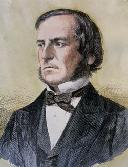
\includegraphics{Boole.jpg}
\end{center}

\href{https://fr.wikipedia.org/wiki/George_Boole}{George Boole}
(\emph{1815-1864}): mathématicien, logicien britannique, auteur d'une
algèbre \textbf{binaire} dite \textbf{booléenne} n'acceptant que deux
valeurs 0 et 1.\\
\href{https://www.dailymotion.com/video/x71hxwp}{Lien} vers la
présentation de Marie Duflot-Kremer, chercheuse en informatique
l'Université de Lorraine.\\
Aujourd'hui, l'algèbre de Boole trouve de nombreuses applications en
informatique et dans la conception des circuits électroniques

    \hypertarget{quelques-duxe9finitions}{%
\section{Quelques définitions}\label{quelques-duxe9finitions}}

On appelle \textbf{valeur logique} ou \textbf{valeur booléenne} toute
valeur notée par deux symboles. On peut utiliser par exemple un des
couples de valeurs suivants : \{0,1\}, \{vrai, faux\}, \{true, false\}
ou \{ouvert, fermé\}.\\
\emph{Exemple}: l'état d'un interrupteur a une valeur booléenne, il peut
être \emph{ouvert} ou \emph{fermé}.

Une \textbf{variable booléenne} (ou variable logique) est une grandeur
représentée par un nom et pouvant prendre une valeur booléenne.\\

L'algèbre de Boole est caractérisée par la donnée:
\begin{itemize}
\item de deux opérations binaires \textbf{OU} et \textbf{ET}
(\emph{correspondant à la somme ``+'' et au produit ``.''})
\item d'une opération unaire \textbf{NON} (\emph{correspondant au
complémentaire \(\ \bar{}\ \)}).
\end{itemize}
Ces opérations doivent vérifier certaines conditions qui ne seront pas
exposées ici. En mathématique on trouve aussi les notations \(\lor\)
(\emph{disjonction}), \(\wedge\) (\emph{conjonction}) et \(\lnot\)
(\emph{négation}).\\

L'association de variables booléennes et d'opérateur(s) booléen(s)
produit une \textbf{expression booléenne}.\\
\emph{Exemple}: si \(a\), \(b\) et \(c\) sont trois variables
booléennes, \(a\cdot b\cdot \bar{c}+a\cdot \bar{b}\cdot c\) est une
expression booléenne.\\

Dresser la \textbf{table de vérité} d'une expression booléenne signifie
construire une table ayant autant de colonnes que de variables d'entrée
plus une colonne donnant le résultat (\emph{vrai} ou \emph{faux}, 0 ou
1) pour chaque combinaison possible des variables d'entrée.

    \hypertarget{les-opuxe9rations-logiques-uxe9luxe9mentaires}{%
\section{Les opérations logiques
élémentaires}\label{les-opuxe9rations-logiques-uxe9luxe9mentaires}}

\hypertarget{les-symboles}{%
\subsection{Les symboles}\label{les-symboles}}

Les opérations logiques sont réalisées simplement avec des circuits
électroniques (à base de transistors) appelés \textbf{portes logiques}.
Voici les symboles des portes logiques utilisées pour les opérations ET,
OU et NON.
\begin{figure}[h]
	\begin{center}
\begin{tabular}{|m{1.5cm}||m{4.5cm}|m{4.5cm}|}
	\hline
	Type & Symbole US & Symbole EU\\
	\hline
	ET& 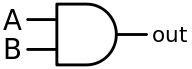
\includegraphics{192px-And.svg.png} &  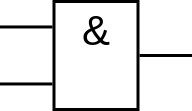
\includegraphics{192px-IEC_AND.svg.png}\\
	\hline
	OU & 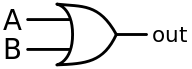
\includegraphics{192px-Or-gate-en.svg.png} &  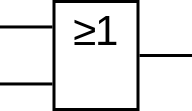
\includegraphics{192px-IEC_OR.svg.png}\\
	\hline
	NON &  
\includegraphics{192px-Not-gate-en.svg.png} &  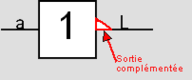
\includegraphics{192px-IEC_Not-gate.png}\\
	\hline
\end{tabular}
\end{center}
\end{figure}

\emph{Note}: les symboles \emph{EU} sont très peu utilisés (même en France!). 

\hypertarget{simulations}{%
\subsection{Simulations}\label{simulations}}
\hypertarget{e1c3}{%
\subsubsection{E1C3 Opérateurs et, ou et non}\label{e1c3}}
Simuler avec le logiciel \emph{Digital} du \href{https://github.com/hneemann/Digital}{professeur Helmut Neemann} les opérations logiques ET, OU et NON. Établir leur table de vérité.

\hypertarget{e2c3}{%
\subsubsection{E2C3 Lois de De Morgan}\label{e2c3}}
\begin{enumerate}
\item Dresser la table de vérité de l'expression \(\overline{A+B}\)
\item Vérifier les résultats par simulation
\item Proposer une expression équivalente
\item Reprendre les questions 1, 2 et 3 avec l'expression \(\overline{A\cdot B}\)
\end{enumerate}

\hypertarget{e3c3-une-opuxe9ration-logique-truxe8s-utilisuxe9e}{%
\subsubsection{E3C3 Une opération logique très
utilisée}\label{e3c3-une-opuxe9ration-logique-truxe8s-utilisuxe9e}}

\begin{enumerate}
\item Ouvrir le circuit ``Dilemme.dig'' (voir fig. \ref{fig:dilemme})

\begin{figure}[!h]
	\begin{center}
		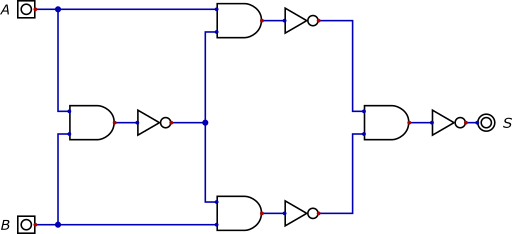
\includegraphics{Dilemme.png}
	\end{center}
	\caption{Fig. \ref{fig:dilemme} -- Dilemme!}
	\label{fig:dilemme}
\end{figure}

\item Réaliser la simulation. Établir et commenter sa table de vérité.
Cette opération très utilisée, appelée \textbf{ OU Exclusif} (voir fig. \ref{fig:xor}) a pour symbole (\emph{US}):\\
\begin{figure}[!h]
	\begin{center}
		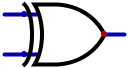
\includegraphics{ouex.png}
	\end{center}
	\caption{Fig. \ref{fig:xor} -- Ou exclusif}
	\label{fig:xor}
\end{figure}
\end{enumerate}

    \hypertarget{probluxe8mes}{%
\section{Problèmes}\label{probluxe8mes}}

\hypertarget{p1c3-addition-binaire}{%
\subsection{P1C3 Addition binaire}\label{p1c3-addition-binaire}}

\hypertarget{demi-additionneur}{%
\subsubsection{Demi additionneur}\label{demi-additionneur}}

Le demi additionneur fig. \ref{fig:halfAdder} est un circuit combinatoire qui permet de réaliser
la somme arithmétique de deux nombres A et B chacun sur un bit. \`A la sortie on va avoir la somme S et une éventuelle retenue R.
\begin{figure}[h]
	\begin{center}
		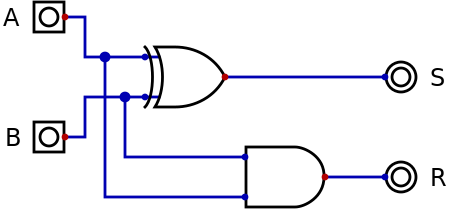
\includegraphics{halfAdder.png}
	\end{center}
	\caption{Fig. \ref{fig:halfAdder} -- Demi additionneur}
	\label{fig:halfAdder}
\end{figure}
\begin{enumerate}
\item Ouvrir le fichier \texttt{halfAdder.dig} et passer en mode simulation.
\item Dresser alors la table de vérité de ce circuit.
\item En déduire la table d'addition binaire.
\item En utilisant la fonction d'analyse du logiciel, donner l'expression
booléenne de la sortie S et de la retenue R
\end{enumerate}

\hypertarget{additionneur-complet}{%
\subsubsection{Additionneur complet}\label{additionneur-complet}}

Lorsqu'on souhaite effectuer l'addition binaire sur un bit de deux
nombres \(A_i\) et \(B_i\), il faut tenir compte d'une éventuelle
retenue \(R_{i-1}\) provenant du calcul du rang précédent. On a alors un
additionneur complet, qui est réalisé avec deux demi-additionneurs (voir fig. \ref{fig:fullAdder}). \`A la sortie on va avoir la somme \(S_i\) et une éventuelle retenue
\(R_i\).
\begin{figure}[h]
	\begin{center}
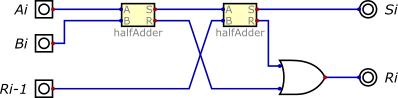
\includegraphics{fullAdder.png}
\end{center}
	\caption{Fig. \ref{fig:fullAdder} -- Additionneur complet}
	\label{fig:fullAdder}
\end{figure}
A la sortie on va avoir la somme \(S_i\) et une éventuelle retenue
\(R_i\).
\begin{enumerate}
\item Ouvrir le fichier \texttt{fullAdder.dig} et passer en mode simulation.
\item Dresser la table de vérité de l'additionneur complet.
\end{enumerate}

\hypertarget{additionneur-complet-en-python}{%
\subsubsection{Additionneur complet en
python}\label{additionneur-complet-en-python}}

Python possède un type booléen nommé \texttt{bool}. Cependant, les
valeurs booléennes \texttt{True} et \texttt{False} peuvent être associées
aux entiers 1 et 0. On peut le vérifier sur l'exemple suivant:

    \begin{Verbatim}[commandchars=\\\{\}]
{\color{incolor}In [{\color{incolor}45}]:} \PY{n}{A} \PY{o}{=} \PY{k+kc}{True}
         \PY{n}{B} \PY{o}{=} \PY{k+kc}{False}
         \PY{n+nb}{print}\PY{p}{(}\PY{l+s+s2}{\PYZdq{}}\PY{l+s+s2}{A == 1 ? : }\PY{l+s+s2}{\PYZdq{}}\PY{p}{,} \PY{n}{A} \PY{o}{==} \PY{l+m+mi}{1}\PY{p}{)}
         \PY{n+nb}{print}\PY{p}{(}\PY{l+s+s2}{\PYZdq{}}\PY{l+s+s2}{B == 1 ? : }\PY{l+s+s2}{\PYZdq{}}\PY{p}{,} \PY{n}{B} \PY{o}{==} \PY{l+m+mi}{1}\PY{p}{)}
         \PY{n+nb}{print}\PY{p}{(}\PY{l+s+s2}{\PYZdq{}}\PY{l+s+s2}{B == 0 ? : }\PY{l+s+s2}{\PYZdq{}}\PY{p}{,} \PY{n}{B} \PY{o}{==} \PY{l+m+mi}{0}\PY{p}{)}
\end{Verbatim}

    \begin{Verbatim}[commandchars=\\\{\}]
A == 1 ? :  True
B == 1 ? :  False
B == 0 ? :  True

    \end{Verbatim}

    L'expression booléenne de la sortie \(S_i\) de l'additionneur complet
est:
\[S_i=(\overline{A_i} \cdot \overline{Bi} \cdot R_{i-1}) + (\overline{A_i} \cdot B_i \cdot \overline{R_{i-1}}) + (A_i \cdot \overline{B_i} \cdot \overline{R_{i-1}}) + (A_i \cdot B_i \cdot R_{i-1})\]
Celle de la retenue est:
\[R_i=(A_i \cdot R_{i-1}) + (A_i \cdot B_i) + (B_i \cdot R_{i-1})\]
En python, les opérateurs booléens sont: \texttt{and}, \texttt{or} et
\texttt{not}. Ainsi l'expression booléenne
\(\overline{A}\cdot(B+\overline{C})\) se traduit par:

\begin{Shaded}
\begin{Highlighting}[]
\KeywordTok{not}\NormalTok{ A }\KeywordTok{and}\NormalTok{ (B }\KeywordTok{or} \KeywordTok{not}\NormalTok{ C)}
\end{Highlighting}
\end{Shaded}
\emph{Remarque}: une expression du type 
\begin{Shaded}
\begin{Highlighting}[]
\NormalTok{ expr1 }\KeywordTok{and }\NormalTok{expr2}
\end{Highlighting}
\end{Shaded}
ou 
\begin{Shaded}
\begin{Highlighting}[]
\NormalTok{expr1 }\KeywordTok{or }\NormalTok{expr2}
\end{Highlighting}
\end{Shaded}
conduit à une évaluation séquentielle c'est-à-dire que python va évaluer $expr1$ puis suivant sa valeur, va évaluer ou non $expr2$. Voyez-vous pourquoi? \par
On définit une fonction en python ayant le code suivant:

    \begin{Verbatim}[commandchars=\\\{\}]
{\color{incolor}In [{\color{incolor}51}]:} \PY{k}{def} \PY{n+nf}{addb}\PY{p}{(}\PY{n}{n}\PY{p}{,}\PY{n}{a}\PY{p}{,}\PY{n}{b}\PY{p}{)}\PY{p}{:}
             \PY{l+s+sd}{\PYZdq{}\PYZdq{}\PYZdq{}}
         \PY{l+s+sd}{    Retourne ....}
         \PY{l+s+sd}{    On suppose que a et b sont des chaines constitués des caractères }
         \PY{l+s+sd}{    appartenant à \PYZob{}\PYZsq{}0\PYZsq{},\PYZsq{}1\PYZsq{}\PYZcb{}; n est un entier naturel supérieur à zéro.}
         \PY{l+s+sd}{    \PYZdq{}\PYZdq{}\PYZdq{}}
             \PY{n}{ri\PYZus{}1} \PY{o}{=} \PY{k+kc}{False}
             \PY{n}{res} \PY{o}{=} \PY{l+s+s2}{\PYZdq{}}\PY{l+s+s2}{\PYZdq{}}
             \PY{k}{for} \PY{n}{i} \PY{o+ow}{in} \PY{n+nb}{range}\PY{p}{(}\PY{n}{n}\PY{o}{\PYZhy{}}\PY{l+m+mi}{1}\PY{p}{,}\PY{o}{\PYZhy{}}\PY{l+m+mi}{1}\PY{p}{,}\PY{o}{\PYZhy{}}\PY{l+m+mi}{1}\PY{p}{)}\PY{p}{:}
                 \PY{n}{ai} \PY{o}{=} \PY{n+nb}{int}\PY{p}{(}\PY{n}{a}\PY{p}{[}\PY{n}{i}\PY{p}{]}\PY{p}{)}
                 \PY{n}{bi} \PY{o}{=} \PY{n+nb}{int}\PY{p}{(}\PY{n}{b}\PY{p}{[}\PY{n}{i}\PY{p}{]}\PY{p}{)}
                 \PY{n}{si} \PY{o}{=} \PY{p}{(}\PY{o+ow}{not} \PY{n}{ai} \PY{o+ow}{and} \PY{o+ow}{not} \PY{n}{bi} \PY{o+ow}{and} \PY{n}{ri\PYZus{}1}\PY{p}{)} \PY{o+ow}{or} \PY{p}{(}\PY{o+ow}{not} \PY{n}{ai} \PY{o+ow}{and} \PY{n}{bi} \PY{o+ow}{and} \PY{o+ow}{not} \PY{n}{ri\PYZus{}1}\PY{p}{)} \PY{o+ow}{or} \PYZbs{}
                 \PY{p}{(}\PY{n}{ai} \PY{o+ow}{and} \PY{o+ow}{not} \PY{n}{bi} \PY{o+ow}{and} \PY{o+ow}{not} \PY{n}{ri\PYZus{}1}\PY{p}{)} \PY{o+ow}{or} \PY{p}{(}\PY{n}{ai} \PY{o+ow}{and} \PY{n}{bi} \PY{o+ow}{and} \PY{n}{ri\PYZus{}1}\PY{p}{)}
                 \PY{n}{ri\PYZus{}1} \PY{o}{=} \PY{p}{(}\PY{n}{ai} \PY{o+ow}{and} \PY{n}{ri\PYZus{}1}\PY{p}{)} \PY{o+ow}{or} \PY{p}{(}\PY{n}{ai} \PY{o+ow}{and} \PY{n}{bi}\PY{p}{)} \PY{o+ow}{or} \PY{p}{(}\PY{n}{bi} \PY{o+ow}{and} \PY{n}{ri\PYZus{}1}\PY{p}{)}
                 \PY{n}{res} \PY{o}{=} \PY{n+nb}{str}\PY{p}{(}\PY{n+nb}{int}\PY{p}{(}\PY{n}{si}\PY{p}{)}\PY{p}{)} \PY{o}{+} \PY{n}{res}
             \PY{k}{if} \PY{n}{ri\PYZus{}1}\PY{p}{:}
                 \PY{n}{res} \PY{o}{=} \PY{l+s+s1}{\PYZsq{}}\PY{l+s+s1}{1}\PY{l+s+s1}{\PYZsq{}} \PY{o}{+} \PY{n}{res}
             \PY{k}{return} \PY{n}{res}
\end{Verbatim}

    \begin{enumerate}
\tightlist
\item
  Consulter la
  \href{https://docs.python.org/fr/3/library/stdtypes.html?highlight=range\#range}{documentation
  officielle} de python sur la fonction \texttt{range} afin de comprendre la
  construction qui apparait à la ligne 9.
\item
  Les spécifications étant incomplètes, expliquer ce que réalise cette
  fonction.
\item
  Vérifier vos hypothèses avec quelques tests; par exemple:
  \begin{itemize}
\item
  \texttt{addb(4,\textquotesingle{}0001\textquotesingle{},\textquotesingle{}0001\textquotesingle{})}
\item
  \texttt{addb(8,\textquotesingle{}11111111\textquotesingle{},\textquotesingle{}00000001\textquotesingle{})}
  \end{itemize}
\item
  Quelle est l'utilité du test ligne 16 ?
\end{enumerate}

    \hypertarget{p2c3-un-circuit-important-le-multiplexeur-pour-les-plus-rapides-et-curieux}{%
\subsection{\texorpdfstring{P2C3 Un circuit important: le multiplexeur
(\emph{pour les plus rapides ET
curieux})}{P2C3 Un circuit important: le multiplexeur (pour les plus rapides ET curieux)}}\label{p2c3-un-circuit-important-le-multiplexeur-pour-les-plus-rapides-et-curieux}}

Le \href{https://fr.wikipedia.org/wiki/Multiplexeur}{multiplexeur} est
un circuit logique très important en architecture machine. Il permet de
sélectionner une entrée parmi \(N\) et de transférer sa valeur sur la
sortie. La sélection se fait à l'aide d'une entrée \emph{Select}.

\hypertarget{principe}{%
\subsubsection{Principe}\label{principe}}

La figure \ref{fig:mux} présente le schéma de principe d'un multiplexeur à
4 entrées \(A_0 ... A_3\) ainsi que sa réalisation avec les portes
logiques élémentaires.
\begin{figure}[h]
	\begin{center}
		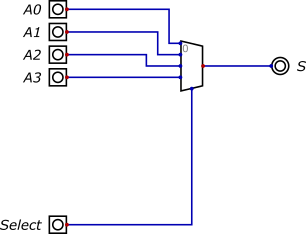
\includegraphics{mux1.png}
		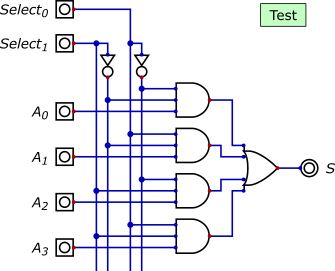
\includegraphics{mux2.png}
	\end{center}
	\caption{Fig. \ref{fig:mux} -- Multiplexeur}
	\label{fig:mux}
\end{figure}	
\hypertarget{simulation}{%
\subsubsection{Simulation}\label{simulation}}

\begin{enumerate}
%\tightlist
\item
  Ouvrir le fichier \texttt{mux2.dig} et passer en mode simulation.
\item
  On souhaite sélectionner la deuxième entrée, quelle valeur logique doit-on affecter à \(Select_0\) et \(Select_1\)?
\item
  Réaliser la sélection précédente. Entrer la combinaison \((1,1,0,0)\)
  pour \((A_0,A_1,A_2,A_3)\). Que vaut \(S\) ? Expliquer.
\item
  Garder la même sélection. Donner une combinaison qui conduit à
  \(S=1\). Expliquer.
\end{enumerate}

    \hypertarget{uxe0-retenir}{%
\section{À retenir}\label{uxe0-retenir}}

L'algèbre de Boole est caractérisée par les trois opérations OU, ET et
NON. Avec ces opérateurs et des variables booléennes on peut construire
des expressions logiques.\\
Dresser la table de vérité d'une expression signifie construire un
tableau qui donne la valeur logique de l'expression pour chaque
combinaison des variables d'entrées.\\
Quelques résultats importants:

	\begin{center}
\begin{tabular}{|c|c||c|c|c|}
	\hline
	A & B & A OU B & A ET B& NON A\\
	\hline
	0 & 0 & 0 & 0 & 1\\
	\hline
	0 & 1 & 1 & 0 & 1\\
	\hline
	1 & 0 & 1 & 0 & 0\\
	\hline
	1 & 1 & 1 & 1 & 0\\
	\hline
\end{tabular}
\end{center}
\vspace{1cm} 
    Ce(tte) œuvre est mise à disposition selon les termes de la Licence
\href{https://creativecommons.org/licenses/by-nc/4.0/}{Creative Commons Attribution - Pas d'Utilisation Commerciale 4.0
International.}
\begin{center}

\includegraphics{Cc-by-nc_icon.svg.png}
\end{center}    
    \end{document}
